\newpage
\section{Discontinuous Galerkin Method}

The Discontinuous Galerkin Method is a method of resolving differential equations through a mesh. It is similar to the Finite Element Method and the Finite Volume Method. This section is for the reader with a beginner's understanding of the Finite Element Method.

\subsection{Basic Overview}


\begin{figure}[ht]
\centering
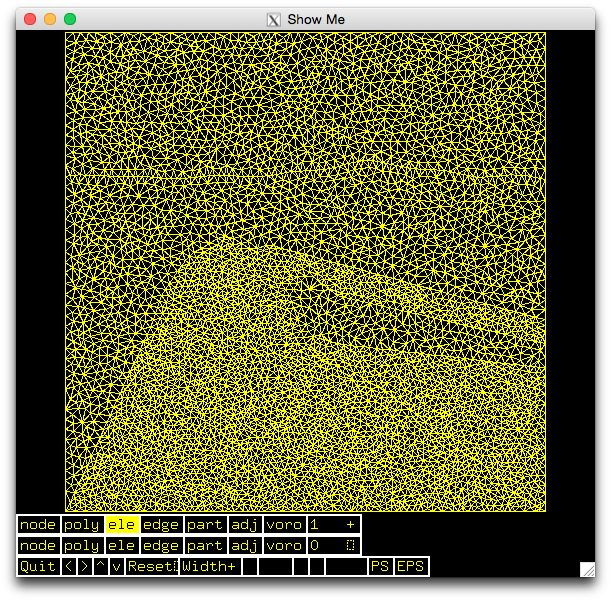
\includegraphics[width=0.7\textwidth]{Images/Example-Mesh.png}
\caption{Example Mesh used to cover example data}
\label{fig:couches5-mesh}
\end{figure}

"Solving differential equations" (such as the acoustic wave equation) is a term that is commonly thrown around without much attention to the essential components in numerical analysis. For the common case, it means: \textbf{given a domain} (for example $[0,10]$ in one dimension or the unit sphere in three dimensions), we \textbf{take a mesh} (set of segments, triangles, tetrahedrons, etc) that covers the domain, and find the values of the variable we are solving for at \textbf{certain moments in time} and at \textbf{certain points in the domain} that are determined by the mesh.

The Discontinuous Galerkin Method is a method frequently used to "solve differential equations". It can be considered a combination of Finite Element Methods (Continuous Galerkin) and Finite Volume Methods. In other words, Discontinuous Galerkin methods are finite element methods that use discontinuous basis functions, thus acquiring more robustness for discontinuous processes. Because the base function polynomials are discontinuous and do not extend over a large stencil,the  Discontinuous Galerkin Method is easily parallelized, and the Mass Matrix is able to be inverted by blocks. Like the Finite Volume Methods, Discontinuous Galerkin methods calculate surface integrals and fluxes of discontinuous terms.

\subsection{Basis Functions}

In Discontinuous Galerkin Methods, we can raise the accuracy of our solution by increasing the order of the polynomials that approximate it. 

The way we represent our solution to the differential equation, is a group of polynomials for each element in the mesh; each polynomial takes a value of $1$ at a certain point called a node, and $0$ at all the other nodes defined in the element. Each base function is discontinuous in that it can take nonzero values inside its own element, but takes the value $0$ on other elements. This is the reason the method is called Discontinuous Galerkin and also the fundamental reason it is easily parallelizable. We can thus define the solution as the linear combination of those functions:

$$u(x,t) = \sum\limits_{i=1}^n c_i(t)\phi_i(x)$$ 
where $c_i(t)$ is merely a time-dependent coefficient and $\phi_i(x)$ is the space-dependent base function defined solely on its corresponding element.


But an important observation that helps us significantly speed up the computation is realizing that we can perform all our integrals on a simple reference element, and then map it onto the actual element. Refer to Figure ~\ref{fig:Reference-Elements} for the visual definition of the reference element in 2 and 3 dimensions as well as the transformation mapping. Here we let the use of the hat in $\hat{E}$ represent the reference element, and the lack of use represent the actual element.


\begin{figure}[ht]
	\centering
	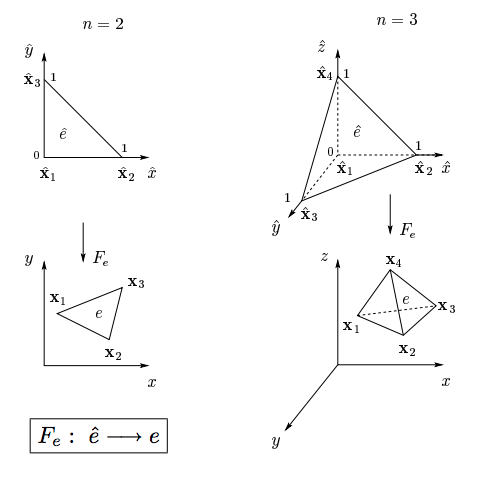
\includegraphics[width=0.7\textwidth]{Images/Reference-Elements.png}
	\caption{Reference Elements transformed to the actual Elements}
	\label{fig:Reference-Elements}
\end{figure}


Given an order $p$, the specific nodes on the reference element are defined as:

$$(\hat{x_i}, \hat{y_j}, \hat{z_k}) = \left( \frac{i}{p}, \frac{j}{p}, \frac{k}{p} \right) \text{ for each } (i,j,k) \in \mathbb{N}^3 \mid i + j + k \leq p$$ 

and we represent the $l$'th node location as $x_l$.

In order to calculate the base functions for the arbitrary order $p$, we can use linear algebra. Namely, we wish to find the base function polynomials of the form:

$$\sum\limits_{i+j+k \leq p} C_{i,j,k} x^i y^j z^k = \sum\limits_{j=1}^n C_j m_j(x)$$
where we have $n$ nodes, $n$ polynomials, and $n$ monomials per polynomial. 

Because the $i$'th polynomial takes a value of $1$ at the $i$'th node and $0$ at all the others, we can represent this relationship with a matrix equation, where the vector on the right is the $i$'th unit vector:

$$\begin{bmatrix}
m_1(x_1) & m_2(x_1) & \ldots & m_n(x_1) \\
m_1(x_2) & m_2(x_2) & \ldots & m_n(x_2)\\
m_1(x_3) & m_2(x_3) & \ldots & m_n(x_3) \\
\ldots   & \ldots   & \ldots & \ldots \\
m_1(x_n) & m_2(x_n) & \ldots & m_n(x_n) 
\end{bmatrix} 
\begin{bmatrix}
C_1 \\
C_2 \\
C_3 \\
\ldots \\
C_n
\end{bmatrix}
= \begin{bmatrix}
0 \\
\ldots \\
1 \\
\ldots \\
0
\end{bmatrix} $$

We can find the polynomial by computing the values of $C_j$,
and summing their product with their corresponding monomials. For simplicity, represent the equation as $S \boldsymbol{C} = \boldsymbol{I}$. By multiplying both sides by $S^{-1}$, we have that $\boldsymbol{C}$ is equal to the $i$'th column of of $S^{-1}$. Thus, we have our $i$'th base function polynomial.

We will go into more depth about how to leverage the linear transformation between the reference element and the actual element in Section ~\ref{subsec: Transformation}. In fact, the method depends on the integral, especially on gradients, laplacians, and partial derivatives.

\subsection{Variational / Weak Formulation}

In order to begin analyzing the acoustic wave equation, we multiply the equation by a test function $v(x,t)$. Do not worry too much about the purpose of the test function, a short summary is that without it, there is no guarantee of finding a function that satisfies the equation. Then we integrate over each element $E$:

\begin{equation} 
\int_E \nabla \cdot \nabla u(x,t) v(x,t) dV + \int_E \frac{\partial^2 u(x,t)}{\partial t^2} v(x,t) dV = \int_E f(x,t) v(x,t) dV 
\end{equation}

Frequently, we need to decompose the integral of the laplacian operator $\nabla \cdot \nabla$ on the domain of the element into an integral on the domain of the element's boundary face in order to place Absorbing Boundary Conditions (new set of differential equations) on the boundary face. In order to do that, we apply Green's first identity to obtain:

\begin{equation}
\int_{\Gamma_E} c^2 v(x,t) \nabla u(x,t) \cdot dS - \int_E c^2 \nabla u(x,t) \cdot \nabla v(x,t) dV - \int_E \frac{\partial^2 u(x,t)}{\partial t^2} v(x,t) dV = \int_E f(x,t) v(x,t) dV
\label{eq:Variational-Form}
\end{equation}

where $\Gamma_E$ is the faces of the element $E$.

\subsection{Mass, Stiffness, Damping Matrices}

We desire to rewrite Equation ~\ref{eq:Variational-Form} in terms of matrices. Specifically, we wish to write it as:

\begin{equation}
\mathcal{M} \frac{\partial^2}{\partial t^2} U_h + c \mathcal{B} \frac{\partial}{\partial t} U_h + c^2 \mathcal{K} U_h = -\mathcal{F}
\label{eq:Matrix-Form}
\end{equation}


The Mass Matrix $\mathcal{M}$ is defined as the matrix in front of the $\frac{\partial^2}{\partial t^2}$ term. The Damping Matrix $\mathcal{B}$ is defined as the matrix in front of the $\frac{\partial}{\partial t}$ term. The Stiffness Matrix $\mathcal{K}$ is defined as the matrix in front of the term with no $t$ at all. 

We also rewrite $u(x,t)$ as its discontinuous space-dependent parts and time dependent parts:
\begin{equation}
u(x,t) = c_1(t) \phi_1(x) + c_2(t) \phi_2(x) + \ldots + c_n(t) \phi_n(x)
\end{equation}

where \begin{equation}
U_h = \begin{bmatrix}
c_1(t) \\
c_2(t) \\
\ldots \\
c_n(t)
\end{bmatrix}
\end{equation}

With this method, we can then transform the equations into a discretized linear matrix form. We will go over this in detail later. 


\subsection{Mass Matrix Calculation}

We begin with the formula below, and attempt to transform it into a matrix form.

\begin{equation}
\int_E \frac{\partial^2 u(x,t)}{\partial t^2} v(x,t) dV
\end{equation}

We want the equalities to be satisfied for any $v(x,t)$ in our function space, so we just need to make sure that the equalities are satisfied for $v(x,t) = \phi_i(x)$ for all $i$. We can do this by using vector and matrix operations to represent multiple equations.

\begin{equation}
\begin{bmatrix}
\int u(x,t) \phi_1 dV \\
\int u(x,t) \phi_2 dV \\
\ldots \\
\int u(x,t) \phi_n dV
\end{bmatrix}
\end{equation}

\begin{equation}
= \begin{bmatrix}
\int \phi_1 \sum\limits_{i=1}^n \frac{\partial^2 c_i(t)}{\partial t^2} \phi_i dV \\
\int \phi_2 \sum\limits_{i=1}^n \frac{\partial^2 c_i(t)}{\partial t^2} \phi_i dV \\
\ldots \\
\int \phi_n \sum\limits_{i=1}^n \frac{\partial^2 c_i(t)}{\partial t^2} \phi_i dV
\end{bmatrix}
\end{equation}

\begin{equation}
= \begin{bmatrix}
\sum\limits_{i=1}^n \frac{\partial^2 c_i(t)}{\partial t^2} \int \phi_1 \phi_i dV \\
\sum\limits_{i=1}^n \frac{\partial^2 c_i(t)}{\partial t^2} \int \phi_2 \phi_i dV \\
\ldots \\
\sum\limits_{i=1}^n \frac{\partial^2 c_i(t)}{\partial t^2} \int \phi_n \phi_i dV
\end{bmatrix}
\end{equation}

\begin{equation}
\label{eq:Mass-Mat}
= \begin{bmatrix}
\int \phi_1 \phi_1 dV & \int \phi_1 \phi_2 dV & \ldots & \int \phi_1 \phi_n dV \\
\int \phi_2 \phi_1 dV & \int \phi_2 \phi_2 dV & \ldots & \int \phi_2 \phi_n dV \\
\ldots                & \ldots                & \ldots & \ldots \\
\int \phi_n \phi_1 dV & \int \phi_n \phi_2 dV & \ldots & \int \phi_n \phi_n dV \\
\end{bmatrix} 
\frac{\partial^2}{\partial t^2} 
\begin{bmatrix}
c_1(t) \\
c_2(t) \\
\ldots \\
c_n(t)
\end{bmatrix}
\end{equation}

\begin{equation}
\label{eq:Mass-Var}
= \mathcal{M} \frac{\partial^2}{\partial t^2} U_h
\end{equation}

where $M$ is the Mass matrix and $U_h$ is the vector of coefficients defining $u(x,t)$. 

The value of the Mass Matrix $\mathcal{M}$ is given by Equation ~\ref{eq:Mass-Mat} and ~\ref{eq:Mass-Var}, and the entry at $(i,j)$ is calculated by:

\begin{equation}
\label{eq:Mass-Eq}
\int_{\hat{E}} \phi_i \phi_j dV
\end{equation}

which is a simple job of integrating multivariate polynomials and can be done by utilizing third party libraries such as SymPy, or by self-coding a polynomial integration system.
 
\subsection{Damping Matrix Calculation}

When using Perfectly Matched Layers, it is no longer necessary to decompose the laplacian to produce a boundary integral. Therefore, we do not have a term with the first derivative of time $\frac{\partial}{\partial t}$, and we do not have a Damping Matrix $\mathcal{A}$.

\subsection{Stiffness Matrix Calculation}

The value of the Stiffness Matrix $\mathcal{B}$ is found through a similar technique. Taking the term with no $t$ at all, we have 
\begin{equation}
\int_E \nabla \cdot \nabla u(x,t) v(x,t) dV
\end{equation}

Once again, we want the equalities to be satisfied for any $v(x,t)$ in our function space, so we just need to make sure that the equalities are satisfied for $v(x,t) = \phi_i(x)$ for all $i$. We can do this by using vector and matrix operations to represent multiple equations.

\begin{equation}
\begin{bmatrix}
\int \nabla \cdot \nabla u(x,t) \phi_1 dV \\
\int \nabla \cdot \nabla u(x,t) \phi_2 dV \\
\ldots \\
\int \nabla \cdot \nabla u(x,t) \phi_n dV
\end{bmatrix}
\end{equation}


\begin{equation}
= \begin{bmatrix}
\int \phi_1 \sum\limits_{i=1}^n c_i(t) \nabla \cdot \nabla \phi_i dV \\
\int \phi_2 \sum\limits_{i=1}^n c_i(t) \nabla \cdot \nabla \phi_i dV \\
\ldots \\
\int \phi_n \sum\limits_{i=1}^n c_i(t) \nabla \cdot \nabla \phi_i dV
\end{bmatrix}
\end{equation}

\begin{equation}
= \begin{bmatrix}
\sum\limits_{i=1}^n c_i(t) \int \phi_1 \nabla \cdot \nabla \phi_i dV \\
\sum\limits_{i=1}^n c_i(t) \int \phi_2 \nabla \cdot \nabla \phi_i dV \\
\ldots \\
\sum\limits_{i=1}^n c_i(t) \int \phi_n \nabla \cdot \nabla \phi_i dV
\end{bmatrix}
\end{equation}

\begin{equation}
\label{eq:Stiff-Mat}
= \begin{bmatrix}
\int \phi_1 \nabla \cdot \nabla \phi_1 dV & \int \phi_1 \nabla \cdot \nabla \phi_2 dV & \ldots & \int \phi_1 \nabla \cdot \nabla \phi_n dV \\
\int \phi_2 \nabla \cdot \nabla \phi_1 dV & \int \phi_2 \nabla \cdot \nabla \phi_2 dV & \ldots & \int \phi_2 \nabla \cdot \nabla \phi_n dV \\
\ldots & \ldots & \ldots & \ldots \\
\int \phi_n \nabla \cdot \nabla \phi_1 dV & \int \phi_n \nabla \cdot \nabla \phi_2 dV & \ldots & \int \phi_n \nabla \cdot \nabla \phi_n dV \\
\end{bmatrix} 
\begin{bmatrix}
c_1(t) \\
c_2(t) \\
\ldots \\
c_n(t)
\end{bmatrix}
\end{equation}

\begin{equation}
\label{eq:Stiff-Var}
= \mathcal{B} U_h
\end{equation}

Thus, by Equations ~\ref{eq:Stiff-Mat}, ~\ref{eq:Stiff-Var} above, we have that the entry at the $(i,j)$ position in the Stiffness Matrix $\mathcal{B}$ is:

\begin{equation}
\label{eq:Stiff-Eq-PML}
\int \phi_i \nabla \cdot \nabla \phi_j dV
\end{equation}



NEW EQUATION BITCH
\begin{equation}
\label{eq:Stiff-Eq-ABC}
\int \nabla \phi_i \cdot \nabla \phi_j dV
\end{equation}

\subsection{RHS Calculation}

The term $\mathcal{F}$ on the right hand side (RHS) is:
\begin{equation}
\begin{bmatrix}
\int f(x,t) \phi_1(x,t) dV \\
\int f(x,t) \phi_2(x,t) dV \\
\ldots \\
\int f(x,t) \phi_n(x,t) dV
\end{bmatrix}
\end{equation}

Given the source function $f(x,t)$, typically a Gaussian distribution multiplied by a Dirac delta function, the integrals in the vector $\mathcal{F}$ are fairly simple to calculate at any given time step. Only the entries in $\mathcal{F}$ that correspond to the element that contains the point source $f(x,t)$ will have integrals that evaluate to non-zero values.

\subsection{Transformation}
\label{subsec: Transformation}

Because we are calculating the terms on the reference element $\hat{E}$ and not on the actual element $E$, we need to be able to map our obtained reference values to actual values. But first, it is necessary to define the linear transformation of the coordinates in terms of matrices and vectors. 

Once again, we reference Figure ~\ref{fig:Reference-Elements} for the definition of $\boldsymbol{\hat{x_1}}, \boldsymbol{\hat{x_2}}, \boldsymbol{\hat{x_3}}, \boldsymbol{\hat{x_4}}, \boldsymbol{x_1}, \boldsymbol{x_2}, \boldsymbol{x_3}, \boldsymbol{x_4}$. Then we have the relation:

\begin{equation}
\label{eq:transform}
\begin{bmatrix}
x \\
y \\
z
\end{bmatrix}
= F_E(\hat{x}, \hat{y}, \hat{z}) = A \begin{bmatrix}
\hat{x} \\ 
\hat{y} \\ 
\hat{z}
\end{bmatrix} + \boldsymbol{b}
= \begin{bmatrix}
x_2-x_1 & x_3-x_1 & x_4-x_1 \\
y_2-y_1 & y_3-y_1 & y_4-y_1 \\
z_2-z_1 & z_3-z_1 & z_4-z_1
\end{bmatrix} \begin{bmatrix}
\hat{x} \\
\hat{y} \\
\hat{z}
\end{bmatrix} + \begin{bmatrix}
x_1 \\
y_1 \\
z_1
\end{bmatrix}
\end{equation}

which we can see as a stretching of the reference element and then translation from $\boldsymbol{\hat{x}}$ to $\boldsymbol{x}$.

Now, when we are changing variables in integrals to determine those integrals on the actual elements, we know that the Jacobian is $|\det A|$


The integrals for which we need to shift coordinates are displayed in Equations ~\ref{eq:Mass-Eq}, ~\ref{eq:Stiff-Eq-ABC}, ~\ref{eq:Stiff-Eq-PML}.

\subsubsection{Mass Entries}

For Equation ~\ref{eq:Mass-Eq} in the calculation of the Mass Matrix, we may simply use the Jacobian that we derived earlier to compute the integral on actual elements:

\begin{equation}
\int_E \hat{\phi}_i \hat{\phi}_j |\det A| dV = |\det A| \int_E \hat{\phi}_i \hat{\phi}_j dV 
\end{equation}

\subsubsection{Stiffness Entries - ABC}

This is slightly more difficult, because we have partial differential forms in the gradient operators. To calculate Equation ~\ref{eq:Stiff-Eq-ABC} on the reference element, we must determine $\nabla \phi(x,y,z) = \left<\frac{\partial \phi}{\partial x}, \frac{\partial \phi}{\partial y}, \frac{\partial \phi}{\partial z}\right>$ in terms of $\nabla \hat{\phi}(\hat{x}, \hat{y}, \hat{z}) = \left<\frac{\partial \phi}{\partial \hat{x}}, \frac{\partial \phi}{\partial \hat{y}}, \frac{\partial \phi}{\partial \hat{z}}\right>$.

\begin{equation}
\nabla \phi(x,y,z) = \begin{bmatrix}
\dfrac{\partial \hat{\phi}(\hat{x}, \hat{y}, \hat{z})}{\partial x} \\
\dfrac{\partial \hat{\phi}(\hat{x}, \hat{y}, \hat{z})}{\partial y} \\
\dfrac{\partial \hat{\phi}(\hat{x}, \hat{y}, \hat{z})}{\partial z}
\end{bmatrix}
\end{equation}

By the chain rule:
\begin{equation}
= \begin{bmatrix}
\dfrac{\partial \hat{\phi}(\hat{x}, \hat{y}, \hat{z})}{\partial \hat{x}} \dfrac{\partial \hat{x}}{\partial x} + \dfrac{\partial \hat{\phi}(\hat{x}, \hat{y}, \hat{z})}{\partial \hat{y}} \dfrac{\partial \hat{y}}{\partial x} + \dfrac{\partial \hat{\phi}(\hat{x}, \hat{y}, \hat{z})}{\partial \hat{z}} \dfrac{\partial \hat{z}}{\partial x} \\
\dfrac{\partial \hat{\phi}(\hat{x}, \hat{y}, \hat{z})}{\partial \hat{x}} \dfrac{\partial \hat{x}}{\partial y} + \dfrac{\partial \hat{\phi}(\hat{x}, \hat{y}, \hat{z})}{\partial \hat{y}} \dfrac{\partial \hat{y}}{\partial y} + \dfrac{\partial \hat{\phi}(\hat{x}, \hat{y}, \hat{z})}{\partial \hat{z}} \dfrac{\partial \hat{z}}{\partial y} \\
\dfrac{\partial \hat{\phi}(\hat{x}, \hat{y}, \hat{z})}{\partial \hat{x}} \dfrac{\partial \hat{x}}{\partial z} + \dfrac{\partial \hat{\phi}(\hat{x}, \hat{y}, \hat{z})}{\partial \hat{y}} \dfrac{\partial \hat{y}}{\partial z} + \dfrac{\partial \hat{\phi}(\hat{x}, \hat{y}, \hat{z})}{\partial \hat{z}} \dfrac{\partial \hat{z}}{\partial z}
\end{bmatrix} 
\end{equation}

\begin{equation}
= \begin{bmatrix}
\dfrac{\partial \hat{x}}{\partial x} & \dfrac{\partial \hat{y}}{\partial x} & \dfrac{\partial \hat{z}}{\partial x} \\
\dfrac{\partial \hat{x}}{\partial y} & \dfrac{\partial \hat{y}}{\partial y} & \dfrac{\partial \hat{z}}{\partial y} \\
\dfrac{\partial \hat{x}}{\partial z} & \dfrac{\partial \hat{y}}{\partial z} & \dfrac{\partial \hat{z}}{\partial z}
\end{bmatrix} \nabla \hat{\phi}(\hat{x}, \hat{y}, \hat{z})
\end{equation}





In order to obtain the value of the matrix above, we look back to the vector Equation ~\ref{eq:transform}.

\begin{equation}
\begin{bmatrix}
x \\
y \\
z
\end{bmatrix}
= A \begin{bmatrix}
\hat{x} \\ 
\hat{y} \\ 
\hat{z}
\end{bmatrix} + \boldsymbol{b}
\end{equation}


Taking the derivative with respect to $x,y,z$, and then multiplying by the inverse of $A$, we get:

\begin{equation}
\newcommand{\dfracstrut}{\vphantom{\dfrac{\partial \hat{x}}{\partial x}}}
A^{-1}\begin{bmatrix}
1 & 0 & 0 \dfracstrut \\
0 & 1 & 0 \dfracstrut \\
0 & 0 & 1 \dfracstrut
\end{bmatrix}
= \begin{bmatrix}
\dfrac{\partial \hat{x}}{\partial x} & \dfrac{\partial \hat{x}}{\partial y} & \dfrac{\partial \hat{x}}{\partial z} \\ 
\dfrac{\partial \hat{y}}{\partial x} & \dfrac{\partial \hat{y}}{\partial y} & \dfrac{\partial \hat{y}}{\partial z} \\ 
\dfrac{\partial \hat{z}}{\partial x} & \dfrac{\partial \hat{z}}{\partial y} & \dfrac{\partial \hat{z}}{\partial z}
\end{bmatrix}
\end{equation}


Transposing gives us the desired matrix so that:

\begin{equation}
\nabla \phi(x,y,z) = A^{-T} \nabla \hat{\phi}(\hat{x}, \hat{y}, \hat{z})
\end{equation}


\subsubsection{Stiffness Entries - PML}
 




\subsection{Time Steps}

Up until now, we have been working out the details of determining the values of $u(x,t)$ in space. Now we work out how to simulate the progression of those values in time. In order to do so, we must use Finite Differences to transform the time derivatives of $u(x,t)$ into more appealing terms using $u(x,t_i)$, the value of $u$ at certain time steps. 

\begin{equation}
\frac{\partial^2}{\partial t^2} u(x,t) \approx \frac{u(x,t+\delta t) - 2 u(x,t) + u(x,t-\delta t)}{\delta t^2}
\end{equation}

\begin{equation}
\frac{\partial}{\partial t} u(x,t) \approx \frac{u(x,t+\delta t) - u(x,t-\delta t)}{\delta t}
\end{equation}




And we are done :)













